\setcounter{chapter}{3}

\chapter{Efficient Coalition Formation for Autonomous Web Services}

\section{Preliminaries}\label{s:preliminaries}

In this section, we discuss the parameters and preliminary
concepts that we use in the rest of the paper.

\subsection{The Architecture}

Our system consists of three main types of entities working
together:

\emph{1) Web services} are rational entities\footnote{The term
rational is used here in the sense that web services are utility
maximizers} providing services to end users. They aim to maximize
their individual income by receiving enough requests from end
users. In order to increase their revenue, web services seek for
more tasks if they have the capacity and throughput to do so. Web
services can join communities to have better efficiency by
collaborating with others, to have access to higher market share,
and to have opportunity of receiving a bigger task pool from end
users. Throughout this paper, in
our equations, we refer to web services as $ws$ and to the set of
web services hosted by a given community as $C$. To simplify the
notation, sometimes we simply write $ws$ instead of $ws \in C$ to
go through the elements $ws$ of the set $C$.

\emph{2) Master Web Services} or the community coordinators, are representatives of the
communities of web services and responsible for their management.
Communities receive requests from users and aim to host a healthy
set of web services to perform the required tasks. They seek to
maximize user satisfaction by having tasks accomplished according
to the desired QoS. In fact, higher user satisfaction will bring
more user requests and increase the market share and revenue of
the community.

\emph{3) Users} generate requests and try to find the best
available services. User satisfaction is abstracted as function of
quantity and quality of tasks accomplished by a given service.
Higher user satisfaction leads to higher trust of the community by users hence directing more requests towards that service provider.

\subsection{Web Service Parameters}\label{ws_parameters}

Web services come with different quality of service parameters.
These parameters with a short description are listed in Table
\ref{qosws}.

\begin{table}[!t]
\centering
\caption{List of web service QoS parameters.}
\begin{tabular}{|c|c||c|c|}
\hline
\textbf{Parameter} & \textbf{Definition} \\
\hline\hline
$Availability$ & Probability of being available during \\
&a time frame \\
$Reliability$ & Probability of successfully handling \\
&requests during a timeframe\\
$Successability$ & Rate of successfully handled requests \\
$Throughput$ & Average rate of handling requests \\
$Latency$ & The average latency of services\\
$Capacity$ & Amount of resources available\\
$Cost$ & Mean service fee \\
$Regulatory$ & Compliance with standards, law and rules\\
$Security$ & Quality of confidentiality \\
&and non-repudiation\\
\hline
\end{tabular}
\label{qosws}
\end{table}


We adopted a real world dataset \cite{DBLP:conf/smc/Al-MasriM09a}
which has aggregated and normalized each of these parameters to a
real value between 0 and 1. Since requests are not shared among
web services and are distributed among all of them inside a
community, each one of them comes with a given QoS denoted by
$(QoS_{ws})$. We assume that $(QoS_{ws})$ is obtained by a certain
aggregation function of the parameters considered in Table
\ref{qosws}. We use this quality output later in evaluating the
community \emph{worth} or \emph{payoff} function.

\subsection{Web Service Communities}\label{webservice-communities}

Figure \ref{fig_community} represents the architecture of web service communities. The communities are essentially an abstract model of web services. They aggregate web services and communicate with other entities such as UDDI registries and users, using identical protocols as web services. Web services join communities to increase their utility by having a larger market share and task pool. Community coordinators or master web services are responsible for community development, managing membership requests from web services and distributing user tasks among the community members. Community coordinators try to attract quality web services and keep the community as stable and productive as possible to gain better reputation and user satisfaction which results in having a higher market share for the community. The way the web services reside inside communities and how communities of web services are engineered is described comprehensively in \cite{DBLP:journals/ijebr/MaamarSTBB09}.

\begin{figure*}[!t]
\centerline{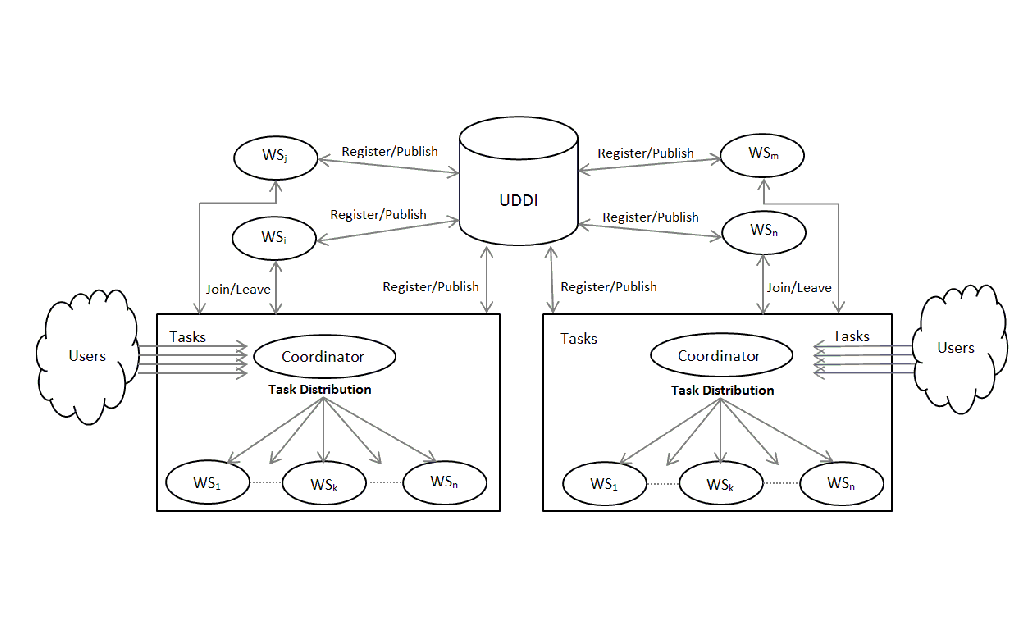
\includegraphics[width=6.25in]{Figures/community.eps}}
\caption{Architecture of Web Service communities}
\label{fig_community}
\end{figure*}








